\chapter{Fabrication}

\section{Overview}
The design of a soft pneumatic actuator is heavily tied to the fabrication process. There are several problems with creating a robot where the bending behavior is highly sensitive to fabrication tolerances. In this work, we were heavily inspired by the fiber reinforced actuators designed by Harvard \cite{galloway_mechanically_2013}. 

\begin{figure}[h]
    \centering
    \includegraphics[width=5 in]{images4/fabricationprocess_0.png}
    \caption{Fabrication process from the Soft Robotics Toolkit}
    \label{fig:toolkitfab}
\end{figure}
% https://softroboticstoolkit.com/book/fr-fabrication

As shown in Figure \ref{fig:toolkitfab}, the robot itself is a hollow tube cast from silicone, where strain limiting materials such as fiberglass and kevlar thread are added to \emph{program} or restrict the strain of the silicone as the we inflate the actuator. After adding the strain limiting materials, we seal the actuator on both ends to create an airtight chamber. Once airtight, we puncture one side to interface with the pressurization equipment that controls the air pressure within the actuator. 

Upon actuation, there are three strains in the material that the fabrication method must keep in mind so that the strains create the desired bending motion. The largest strain is the axial strain. The axial strain is the strain along the length of the actuator. Following the same principles as the standard fiber-reinforced soft pneumatic actuator, using a semi-circular cross section, attaching the fiber glass fabric to the flat side is the easiest way to control axial strain. The fabric cannot strain. The slices of silicone away from the strain limiting fabric are allowed to axially strain, and the top of the semi-circular cross section has the most axial strain. 

Strains in the other axes that also influence the bending behavior of the actuator are considered as losses. Since the bending behavior is primarily defined by the axial strain, any air pressure being converted into circumferential or radial strain is a loss. This is where the kevlar string comes in. To limit circumferential strain, fibers can be wrapped around the outside of the cross section. Based on the angle and amount of times we wrap the actuator with the thread, different types of circumferential strains are allowed. This allows the actuators to bend and coil in different directions upon actuation. 

In the standard actuator, the silicone is cast around a metal rod, and the 3D printed mold has indents to create markers of where to wrap the thread. After wrapping, another thinner layer of silicone is cast over the threads to seal them in. 

Since we wanted to create an actuator with inverted bending behavior, we made the actuator circular. The semi-circular cross section faces the inside such that the flat side is longer and on the exterior. With actuation, the semi-circular section would axially strain around the neutral bending axis of the fiberglass fabric to achieve the unbending behavior. 

Any variations in the cross section along the length would create variation in the all three strains, so the first goal was to fabricate an actuator with a uniform cross section. The dimensions of the desired cross section are shown in Figure \ref{fig:crosssection}.

\begin{figure}[h]
    \centering
    \includegraphics[width=5 in]{images4/cross-section-drawing.jpg}
    \caption{Drawing of the cross section and circular shape of the actuator.}
    \label{fig:crosssection}
\end{figure}

\section{Casting Silicone}
One of the goals of this project was to create an accessible fabrication method, to reduce the complexity of creating a single robot. To create a robot with a circular shape along the length and a uniform semi-circular cross section, we needed a way to cast the silicone around an arch-shaped inner piece, which would be removed to form the hollow chamber. We decided on the open angle of about 35$^\circ$, which determines the total length of the actuator based on the casting process of silicone. If the actuator were to extend further underneath itself, casting vertically would not have been possible. 

First, a little background on silicone casting. The silicones chosen for this project were platinum cure, two part silicones from Smooth-On. We used five different silicones with Shore A Hardness ranging from 20--50: Dragon~Skin~20~(DS20), Dragon~Skin~30~(DS30), Smooth~Sil~940~(SS40), Smooth~Sil~945~(SS45), and Smooth~Sil~950~(SS50). The shore hardness of the actuator can be equated to the bending resistance: the harder the material, more stress is required to achieve a certain strain. Each of these silicones are well mixed, measured by weight, and degassed before pouring into any molds. We started with just using DS20 silicone since it has the fastest cure time, about 4 hours, and it is the easiest to mix of the four silicones. Its important that any materials used during the mixing process are compatible with the silicones and will not impact the curing process. We used popsicle sticks and metal spatulas for mixing within plastic cups. Figure \ref{fig:castingstation} contains an image of the casting station covered in paper as any drips of each part of silicone not mixed properly will never cure and can become quite sticky. 

\begin{figure}[h]
    \centering
    \includegraphics[width=4 in]{images4/castingstation.jpeg}
    \caption{Photo of the casting station featuring Dragon Skin 20 Silicone, the scale and plastic cup for weighting each part of the 2 part silicone.}
    \label{fig:castingstation}
\end{figure}

Once the two parts are mixed together, we degassed in a vacuum chamber for about 2-3 minutes, or until all of the large bubbles of air have been removed. The mixed silicone has the viscosity similar to honey, it is easy to pour but sticks to everything. Its important to remove any air from the silicone as if the silicone cures around the air bubbles, the little pockets ruin the uniform cross section required for consistent bending behavior. 

\section{Arch-Shaped Dies}

When trying to cast this shaped actuator out of a single pour of silicone, the arch shape allows for silicone to be poured in from the top, and with the help of gravity, the silicone flows down to each end of the actuator. 

With the guidance from Cooper's AACE Lab staff, Harrison Tyler and Judy Li, we had access to multiple different filaments and materials for creating the pieces required for casting. The first check with any mold piece not made from PLA, is to ensure that the material does not inhibit the silicone's curing process. Materials with high sulphur content, for example, completely inhibit the curing process. 

We chose to 3D print the outer molds from PLA. The mold has an arch shape so that the actuator can be casted vertically through a large pour hole, and any air would be able to escape from the top of the mold. The insert would slot into the mold so that it would be in the center, creating the even semi-circular cross section. The top of the mold had a large pour hole, and the walls maintained the height of the actuator so that any material attached to the flat side of the actuator could be later removed after the silicone cured. 

\begin{figure}[h]
    \centering
    \includegraphics[width=5 in]{images4/firstmolddesign.jpg}
    \caption{Design for the first mold, left is an isometric view of the 3 pieces, right is a front view of the insert inside one side of the mold.}
    \label{fig:firstmold}
\end{figure}

One side of the mold had feet such that the other side of the mold would fit into it, the molds fit together like puzzle pieces, once again to maintain the constant cross section. Figure \ref{fig:firstmold} contains the first mold designed for casting the circular actuator, highlighting the large pour hole at the top, the slot for the insert to lock into, and the asymmetries at the bottom of the molds so that they fit together and no silicone was allowed to escape from the bottom. 

\section{Dissolvable Inserts}

\begin{figure}[h]
    \centering
    \includegraphics[width=6.5 in]{images4/pvainsert.jpg}
    \caption{Fabrication of PVA inserts: A. PVA insert printed with PLA support material. B. DS20 actuators after removing from mold. C. DS20 and SS45 actuators after removing excess silicone. D. Hollow actuators post hot water bath.}
    \label{fig:pvainsert}
\end{figure}

Commonly used as support material for PLA 3D prints, PVA (Polyvinyl Alcohol) is a filament material that is soluble in water and safe to dispose of. Figure \ref{fig:pvainsert} contains photos of actuators fabricated using a PVA insert.  After confirming that the silicone could cure around this material, we printed the first inserts out of PVA using an Ultimaker 3D printer. Since this material is rigid, only 5-10\% infill was required. The higher the infill on the insert, the more time consuming it would be to remove. For the support material, we used PLA filament. These inserts would be single use, and were removed from the silicone using a hot water bath. Even though there were no problems removing the insert from the silicone post cure, needing to print a new insert for every actuator used a lot of material, and was time consuming. The PLA molds could be used for dozens of actuators but a single-use insert did not align with the goal of simple mass production. To confirm the insert was removable for one of the harder silicones, we casted an SS45 actuator using a PVA insert.  

\section{Flexible Inserts}

At AACE Lab, we had access to TPU (Thermoplastic Polyurethane) filament, which is similar to rubber, its flexible and would be removable after the silicone cured without damage to the silicone. Based on the infill \% chosen, the TPU insert's stiffness could be tuned. The inserts were printed on the bed horizontally with no support material. The overhang created an inconsistent cross section, so we began printing with TPU as support material. The drawback of TPU inserts were that even though they could be used to cast multiple actuators, over time, they would begin to lose their shape. To combat the flexibility of the TPU insert, we used pins to hold the insert in place within the mold. Using 3 sets of pins, we could ensure the TPU insert would remain in the center of the mold so that the cross section of the silicone would be uniform. We used a FormLabs Resin Printer to fabricate the pins. Once again confirming the silicone could cure around the chosen resin, we began casting actuators using the TPU inserts. Figure \ref{fig:tpuinsert} contains photographs of the fabrication process for the first inserts. 

\begin{figure}[h]
    \centering
    \includegraphics[width=6.5 in]{images4/tpuinsertfab.jpg}
    \caption{Fabrication of TPU inserts: A. Molds printed from PLA. B. Solid TPU inserts printed without support material. C. Comparison of different temperature settings on print quality of TPU. D. Resin printed pins of 2 materials. E. TPU insert with holes for the pins and the removed support material. F. TPU insert with pins inside of one half of the mold.}
    \label{fig:tpuinsert}
\end{figure}

The pins created a new problem of needing to patch the holes left behind in the silicone. After casting the actuator with the TPU insert and Pins, a solid TPU insert was reinserted into the hollow silicone so the holes could be patched with more DS20 silicone. Mixing and casting more silicone to patch the holes was not ideal but it allowed us to seal the holes and create an airtight actuator. 

\section{Casting with TPU insert}

Using the TPU insert with the pins to maintain the cross section along the length of the actuator, we were successful at fabricating a few actuators. Photos of the fabrication process are in Figure \ref{fig:tpupinfab} The pour hole for the mold was not large enough for all of the air bubbles to escape the top of the mold, so we cut away a small section in the center of the mold. To fill the mold, we used 40~g of part A and 40~g of part B of the DS20 silicone. To hold the molds together, we used several clamps to minimize flashing of the silicone and ensure the uniform cross section. We poured the silicone in a small amount at a time, ensuring any air bubbles were able to rise to the top. When pouring silicone, if the ribbon of silicone gets too thin, more air is introduced as the silicone folds onto itself. Frequent tapping of the mold on the lab bench was required to ensure all of the air escaped. 

\begin{figure}[h]
    \centering
    \includegraphics[width=6.5 in]{images4/tpupincasting.jpg}
    \caption{Fabrication of the hollow actuator using a TPU insert and pins. A. The pins placed in the insert. B. The clamps placed on the mold with the insert inside. C. Post silicone cure. D. Removing excess silicone. E. Removing the pins and insert. F. Silicone with solid insert. G. Post patching the holes from the pins. H. Completed hollow actuator body.}
    \label{fig:tpupinfab}
\end{figure}

After the silicone cured, we used a sharp blade to cut away any flashing, the silicone at the bottom of each end, and the silicone that remained in the pour hole. After removing the pins and the TPU insert, using a small amount of IPA (isopropyl alcohol) as a lubricant, we inserted the solid TPU so that the holes left behind by the pins could be patched. After cleaning up the ends to make them flat, the hollow actuator is ready for the next steps of the fabrication process, sealing both ends and adding the interface for the pressurization equipment. 

\section{Case Study: SS45 Silicone}

The TPU insert with pins method was successful at creating an airtight actuator for the soft DS20 silicone, so to test if the fabrication procedure would work for stiffer silicones, we casted an actuator out of SS45 silicone. This silicone has a viscosity closer to peanut butter than honey and was laborious to mix and pour. Despite tapping the mold on the lab bench to remove the trapped air bubbles, large bubbles at the top of the mold remained. A bigger issue was that the TPU insert could not be removed. The silicone was too stiff for the end caps of the insert to slide through. We had to cut the silicone to remove the insert. Upon further inspection, a few air pockets remained inside of the silicone. Figure \ref{fig:ss45mess} contains photos of testing the TPU insert and pins fabrication method for SS45 silicone. 

\begin{figure}[h]
    \centering
    \includegraphics[width=6 in]{images4/ss45mess.jpg}
    \caption{Images of failed SS45 actuator casting attempts. A. Overflow of mold during degassing. B. Samples of gaps created by air bubbles stuck in the mold. C. Un-patchable hole left from pin. D. Swiss-cheese actuator from over degassing}
    \label{fig:ss45mess}
\end{figure}

To combat the air holes that remained in the silicone, we attempted to degas the entire mold after casting the actuator. The small air pockets expanded and left the actuator with a consistency of swiss cheese. Additionally, the pins left large holes and since the solid TPU insert could not be slid in to patch the holes, we had to look into alternate methods of restricting the flexible insert. 

\section{Case Study: DS20 Spacers}

For DS20 silicone, patching the holes left behind by the pins was successful at creating an airtight seal. In an attempt to remove the need to patch the holes, we attempted casting actuators using rings of DS20 silicone to hold the TPU insert in place. We printed a mold to cast small semi-circular rings of DS20 silicone, then cut a piece away so while casting the actuator's body, the silicone would flow past the spacers and reach the ends. The placement of the spacers was somewhat arbitrary as we were unsure if this method would create an airtight seal. After casting the actuator and removing from the molds, simply pulling on the actuator would break the seal between the silicone pieces. Figure \ref{fig:ds20spacer} contains images of this attempt at centering the TPU insert inside of the mold. 

\begin{figure}[h]
    \centering
    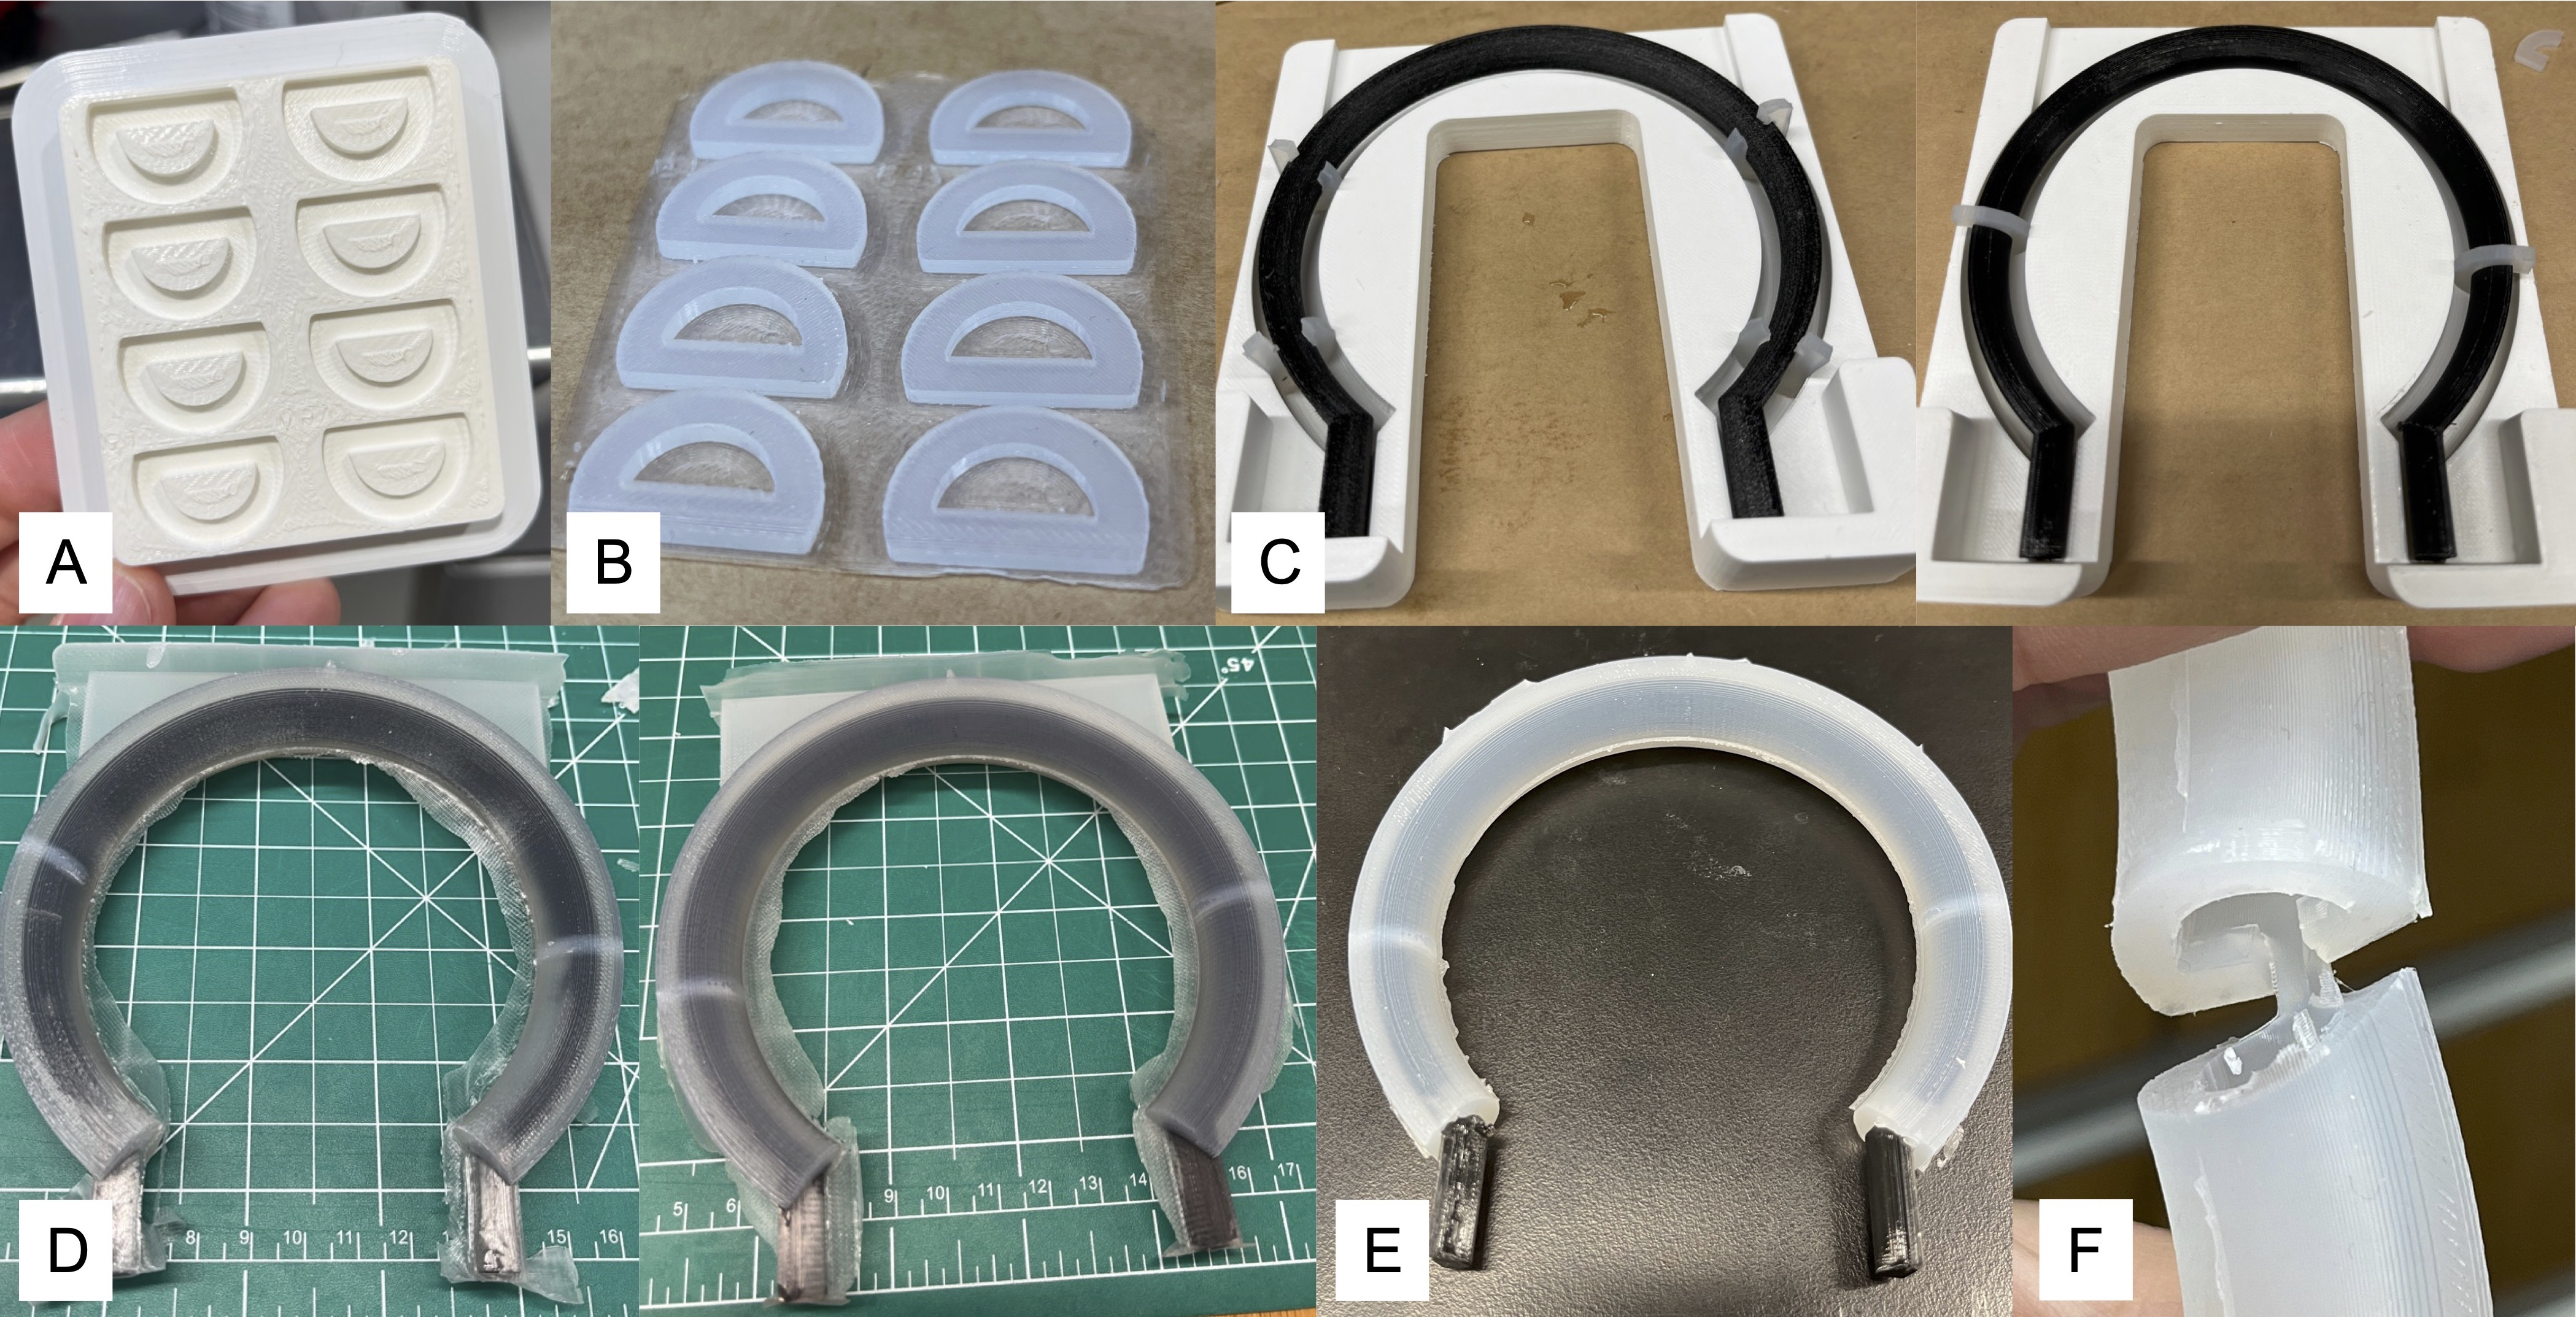
\includegraphics[width=6 in]{images4/ds20spacer.jpg}
    \caption{Images of failed attempts at using a spacer made from DS20 silicone to center the TPU insert. A. 3D printed mold for the spacers. B. casted spacers. C. Arbitrary placement of spacers. D. Casted actuators right after removing from the mold. E. After removing excess silicone. F. Failed attempt at creating a seal.}
    \label{fig:ds20spacer}
\end{figure}

\section{Mold Improvements}
The molds we 3D printed had served us well, but were beginning to buckle from the frequent clamping and tapping on the table to remove air from the actuators. The increase in flashing post each cast meant it was time to print new molds. The first upgrade was a larger pour hole with extra relief for the air bubbles that would get stuck at the top of the mold. Additionally, clamp placement needed to be on the parts where the two halves of the molds touch. If the clamp was tightened around an area meant to be filled with silicone, we noticed that the silicone walls would be uneven. Adding markings for safe places to apply the clamps improved wall thickness significantly. For the thinner silicones, extra clamps on the interior section were required to reduce leakage and flashing, as shown in Figure \ref{fig:newmolds}.

\begin{figure}[h]
    \centering
    \includegraphics[width=6 in]{images4/newmolds.jpg}
    \caption{Upgrades to the molds. A. Drawing of the larger pour hole. B. Drawing of the molds with markings for clamp placement. C. Photo of additional clamps required on the interior.}
    \label{fig:newmolds}
\end{figure}

\section{Case Study: Wax Inserts}

Creating an insert from wax was perhaps more trouble than it was worth, but it did lead us closer to the final fabrication method. We found three waxes compatible with curing silicone: Beeswax, paraffin wax, and microcrystalline wax. To cast the wax insert, we 3D printed a new mold and an insert out of PLA for casting a mold from silicone. We then casted the wax into the silicone mold. 

All three waxes were able to be partially casted and removed from the silicone mold. However, we found that the creating the wax insert to have the perfect cross section shape to ensure a future uniform cross section for the actuator to be difficult and the waxes were not rigid enough to hold their shape inside of the mold during casting. We thought about combining waxes in different ratios to enhance the stiffness and ease of casting, but even if the wax inserts were able to create the perfect cross section when casting silicone, they would have to be melted and recast for fabricating each actuator. With mass production in mind, we decided to not further pursue wax inserts. Figure \ref{fig:waxinserts} contains images from experimenting with wax inserts. 

\begin{figure}[h]
    \centering
    \includegraphics[width=6 in]{images4/waxinserts.jpg}
    \caption{Experimentation with wax inserts. A. 3D printed mold and insert for casting silicone mold for wax. B. Using popsicle sticks to hold insert above silicone while casting mold. C. Paraffin wax casted in silicone mold. D. Paraffin insert removed from mold. E. Beeswax and Microcrystalline wax cast in silicone molds. F. Beeswax and Microcrystalline wax removed from silicone molds}
    \label{fig:waxinserts}
\end{figure}

\section{Case Study: PCL Inserts}

PCL (Polycaprolactone) is a plastic that has a low melting temperature and is moldable with the use of warm water. Using the same silicone mold made for the wax inserts we used warm water to melt the PCL pellets into blobs which were pressed into the silicone mold. The DS20 mold was far too flexible to accurately shape the PCL. Also, as the pieces of PCL cooled and solidified, they would not fully bond with the other pieces, leaving air gaps in the insert. After tuning the timing between the pieces cooling down and adding more PCL pieces we were successful at creating an insert, and cast a DS20 actuator around the PCL insert. Unfortunately, the walls of the silicone were uneven and the PCL insert has the same single use problem as the wax inserts. Figure \ref{fig:pclinsert} contains photographs of experimenting with PCL as an insert and the DS20 actuator we casted using the PCL insert. 

\begin{figure}[h]
    \centering
    \includegraphics[width=6 in]{images4/pclinsert.jpg}
    \caption{Experimentation with PCL inserts. A. Silicone mold. B. An attempt. C. Melting PCL in warm water. D. PCL insert inside PLA mold. E. Casted around PCL insert. F. Removed from mold. G. Extra silicone removed. H. Final actuator.}
    \label{fig:pclinsert}
\end{figure}